% Exposé VI. Extensions and mergeability: Definition VI.1 to Theorem VI.5.
% Sources: theory/framework.md (Exposé VI), site/sections/09-merge.html, theory/propositions.json
% (public statements of VI.2 to VI.5, round-2 repairs). Proofs are in Appendix C.
\section{Extensions and mergeability}\label{sec:merge}

\begin{flushright}\small\itshape
When a lift fails, look for the place where it fails,\\
and give the obstruction a name.\\[3pt]
{\upshape\footnotesize after Grothendieck}
\end{flushright}

Adapters, prefixes, prompts and ReFT enlarge the network before they train, so merging them back is a lifting problem.
Seven local rewrite rules give sufficient conditions for a merge and name the side condition that fails when they stop.

Merging an extension back means finding a weight of the original network that computes the trained function. The rules
slide an edit along the wires of a block until a weight absorbs it. They certify a merge when the edit acts alike at
every position, the absorbing weights are unshared, shifts have bias slots and, under RoPE, scales are constant on rotary
pairs. A stuck rewrite shows only a box-local obstruction. Three examples show what the exposé finds. The feed-forward
scale of (IA)$^3$ always folds into $W_{\mathrm{down}}$; it folds into $W_{\mathrm{up}}$ under SwiGLU for every scale
and under ReLU for nonnegative ones, and under GELU only entries $0$ and $1$ fold. A prefix is a gated parallel adapter
whose gate depends on the input, so for generic frozen weights it cannot be folded into the head's own weights. Per
hidden vector, LoReFT is LoRA on an inserted identity box, and since it acts at selected positions no merge is known.

% ------------------------------------------------------------------------------------------------
\subsubsection{The weight that absorbs the edit}\label{sec:merge-hook}

(IA)$^3$ \citep{liu2022few} rescales the hidden units of a feed-forward block by a learned vector $\ell$, which one
would like to fold into a frozen weight after training. The weight that reads the hidden units, $W_{\mathrm{down}}$,
absorbs $\ell$ under every activation. The weight that produces them, $W_{\mathrm{up}}$, absorbs it under SwiGLU for
every $\ell$, under ReLU when no entry is negative, and under GELU only for entries $0$ or $1$.

The activation belongs to the network, which a weight-space method never sees (\thmref{Remark}{I.3}). Adapters,
prefixes, prompts and ReFT add boxes the pretrained network lacked, and whether they can be removed depends on their
surroundings. Figure~\ref{fig:merge} runs the rules of this exposé on one block.

\begin{figure}[tbp]
\centering
\begin{tikzpicture}[x=1cm,y=1cm,
  wire/.style={inkgray,line width=0.6pt},
  bx/.style={draw=tide,fill=tide!8,rounded corners=1.5pt,minimum height=5.2mm,minimum width=8.5mm,inner sep=2pt,
    font=\footnotesize,text=ink},
  op/.style={draw=inkgray,fill=white,circle,inner sep=0.6pt,minimum size=5.2mm,font=\scriptsize,text=ink},
  nb/.style={draw=inkgray,fill=white,rounded corners=1.5pt,minimum height=5mm,inner sep=2pt,font=\scriptsize,text=ink},
  ed/.style={draw=ochre,fill=ochre!18,diamond,aspect=1.3,inner sep=0.5pt,minimum size=5.6mm,font=\scriptsize,text=ink},
  bad/.style={draw=seal,fill=seal!10,rounded corners=1.5pt,minimum height=5mm,inner sep=2pt,font=\scriptsize,text=ink},
  cp/.style={circle,fill=inkgray,inner sep=0pt,minimum size=3.6pt},
  ok/.style={-{Stealth[length=1.8mm]},moss,line width=0.85pt},
  cond/.style={-{Stealth[length=1.8mm]},ochre,line width=0.85pt},
  no/.style={-{Stealth[length=1.8mm]},seal,line width=0.85pt,dash pattern=on 2.2pt off 1.6pt},
  rl/.style={font=\sffamily\scriptsize,inner sep=1.2pt},
  note/.style={font=\scriptsize,text=inkgray,align=left,inner sep=1pt}]
% ============================================================ (a) attention sublayer
\begin{scope}
\node[anchor=west,font=\small,text=ink] at (-0.25,3.75) {\textbf{(a)} attention sublayer, RoPE};
\draw[wire] (-0.2,0) -- (14.7,0);
\node[note,anchor=north west] at (-0.2,-0.06) {residual stream $h$};
\node[cp] (a0) at (0.5,0) {};
\node[nb] (an) at (1.3,1.9) {$n$};
\node[bx] (ag) at (2.3,1.9) {$\gamma\odot$};
\node[cp] (a1) at (3.2,1.9) {};
\node[bx] (WQ) at (4.2,2.9) {$W_Q$};
\node[bx] (WK) at (4.2,1.9) {$W_K$};
\node[bx] (WV) at (4.2,0.9) {$W_V$};
\node[ed] (lq) at (5.4,2.9) {$\ell$};
\node[ed] (lv) at (5.4,0.9) {$\ell_v$};
\node[op] (Rm) at (6.5,2.9) {$R_m$};
\node[op] (Rn) at (6.5,1.9) {$R_n$};
\node[op] (dot) at (7.6,2.4) {$\langle\,,\rangle$};
\node[nb] (sm) at (8.75,2.4) {softmax};
\node[nb] (mix) at (10.05,1.6) {$\sum_j a_jv_j$};
\node[bx] (WO) at (11.3,1.6) {$W_O$};
\node[ed] (ssf) at (12.45,1.6) {$s,t$};
\node[op] (ap) at (13.1,0) {$+$};
\node[ed,draw=seal,fill=seal!12] (reft) at (14.0,0) {$\Phi$};
\node[bad] (P) at (8.75,3.45) {prefix $P$};
% wires
\draw[wire] (a0) |- (an);
\draw[wire] (an) -- (ag);
\draw[wire] (ag) -- (a1);
\draw[wire] (a1) |- (WQ);
\draw[wire] (a1) -- (WK);
\draw[wire] (a1) |- (WV);
\draw[wire] (WQ) -- (lq);
\draw[wire] (lq) -- (Rm);
\draw[wire] (WK) -- (Rn);
\draw[wire] (WV) -- (lv);
\draw[wire] (Rm) -- (dot);
\draw[wire] (Rn) -- (dot);
\draw[wire] (dot) -- (sm);
\draw[wire] (sm.east) -| (mix.north);
\draw[wire] (lv.east) -| (mix.south);
\draw[wire] (mix) -- (WO);
\draw[wire] (WO) -- (ssf);
\draw[wire] (ssf.east) -| (ap.north);
\draw[seal,line width=0.6pt] (P) -- (sm);
% rewrites
\draw[ok] (lq.north) to[out=105,in=75] node[rl,above,text=moss]{R1} (WQ.north);
\draw[cond] (lq.south west) to[out=-115,in=15] node[rl,right,pos=0.45,text=ochre]{R5} (WK.north east);
\draw[ok] (lv.south) to[out=-105,in=-75] node[rl,below,text=moss]{R1} (WV.south);
\draw[ok] (ag.north) to[out=85,in=175] node[rl,above left,pos=0.2,text=moss]{R7, R6} (WQ.north west);
\draw[cond] (ssf.north) to[out=105,in=75] node[rl,above,text=ochre]{R1} (WO.north);
% labels of blocked edits
\node[note,anchor=west,text=seal] at (P.east) {\ VI.5(f)};
\node[note,anchor=north,text=seal] at (reft.south) {LoReFT, VI.4(c)};
\end{scope}
% ============================================================ (b) feed-forward sublayer
\begin{scope}[yshift=-4.75cm]
\node[anchor=west,font=\small,text=ink] at (-0.25,3.75) {\textbf{(b)} SwiGLU feed-forward sublayer};
\draw[wire] (-0.2,0) -- (14.7,0);
\node[note,anchor=north west] at (-0.2,-0.06) {residual stream $h$};
\node[cp] (b0) at (0.5,0) {};
\node[nb] (bn) at (1.3,2.1) {$n$};
\node[bx] (bg) at (2.3,2.1) {$\gamma\odot$};
\node[cp] (b1) at (3.2,2.1) {};
\node[bx] (Wg) at (4.2,2.9) {$W_g$};
\node[bx] (Wu) at (4.2,1.3) {$W_{\mathrm{up}}$};
\node[op] (sig) at (5.6,2.9) {$\sigma$};
\node[op] (had) at (6.9,2.1) {$\odot$};
\node[ed] (l) at (8.1,2.1) {$\ell$};
\node[bx] (Wd) at (9.4,2.1) {$W_{\mathrm{down}}$};
\node[bad] (ad) at (11.05,2.1) {$\id+U\sigma(D\,\cdot)$};
\node[op] (bp) at (13.1,0) {$+$};
% wires
\draw[wire] (b0) |- (bn);
\draw[wire] (bn) -- (bg);
\draw[wire] (bg) -- (b1);
\draw[wire] (b1) |- (Wg);
\draw[wire] (b1) |- (Wu);
\draw[wire] (Wg) -- (sig);
\draw[wire] (sig.east) -| (had.north);
\draw[wire] (Wu.east) -| (had.south);
\draw[wire] (had) -- (l);
\draw[wire] (l) -- (Wd);
\draw[wire] (Wd) -- (ad);
\draw[wire] (ad.east) -| (bp.north);
% rewrites
\draw[ok] (l.north) to[out=75,in=105] node[rl,above,text=moss]{R1} (Wd.north);
\draw[ok] (l.south) to[out=-90,in=-15] node[rl,below,pos=0.55,text=moss]{R4, then R1} (Wu.south east);
\draw[no] (l.north west) to[out=140,in=10] node[rl,above right,pos=0.18,text=seal]{R3} (sig.north east);
\draw[ok] (bg.north) to[out=85,in=175] node[rl,above left,pos=0.2,text=moss]{R7, R6} (Wg.north west);
% notes
\node[note,anchor=north,text=seal] at (ad.south) {VI.3(c)};
\node[note,anchor=west] at (8.1,0.6) {Here $\sigma=\mathrm{silu}$. In an ungated\\ block, R3 passes a ReLU for $\ell\ge0$;\\ under GELU only $\ell_i\in\{0,1\}$ pass.};
\end{scope}
\end{tikzpicture}
\caption{The merge rules of \thmref{Theorem}{VI.3} on a pre-LN transformer block, drawn as a string diagram with the
residual stream along the bottom: (a) the attention sublayer under RoPE, (b) a SwiGLU feed-forward sublayer. Tide boxes
are trainable boxes of the base network, $\bullet$ is a copy node, $\odot$ the product node of the gated block, and
ochre diamonds are edits inserted by a method. Moss arrows are rewrites licensed for every parameter value, ochre arrows
rewrites licensed under a side condition, and seal marks what the rules do not merge. A query scaling $\ell$ fuses into
$W_Q$ by R1; R5 moves it onto $W_K$ only if $\ell$ is constant on each rotary pair and across a grouped-query sharing
group. A value scaling $\ell_v$ fuses into $W_V$. A norm gain is copied to every reader (R7) and absorbed (R6). SSF's
scale and shift $(s,t)$ fuse into $W_O$ only if $W_O$ has a bias slot. The (IA)$^3$ scale fuses into
$W_{\mathrm{down}}$ (R1), and through the product node into $W_{\mathrm{up}}$ for every $\ell$ (R4, then R1); it does not
slide through the SiLU gate, and in an ungated block R3 carries it through a ReLU only for $\ell\ge0$. A prefix enters the
softmax with an input-dependent gate (\thmref{Theorem}{VI.5}(f)), a nonlinear adapter is a non-affine edit
(\thmref{Theorem}{VI.3}(c)), and LoReFT acts at selected positions of the residual stream
(\thmref{Proposition}{VI.4}(c)); R1--R7 merge none of the three. The companion site's merge game runs these rewrites
interactively, with a float64 check of each licensed merge on seeded weights.}\label{fig:merge}
\end{figure}

% ------------------------------------------------------------------------------------------------
\subsubsection{Extensions, and merging as a lift}\label{sec:merge-extensions}

An adapter $y\mapsto y+U\sigma(Dy)$ \citep{houlsby2019parameter} adds weights $(U,D)$, and at $U=0$ the network
computes the old function. A prefix \citep{li2021prefix} adds key--value pairs to every softmax, and ReFT
\citep{wu2024reft} edits hidden states at chosen positions. Each time $\Theta$ grows to $\Theta\times\Theta'$ and $f$ to
a larger $\tilde f$. A prefix always takes softmax mass, and on a head with $W_oW_v\ne0$ no prefix leaves the output
unchanged, so prefixes have no neutral setting there (\thmref{Theorem}{VI.5}(f)).

\begin{definition}{VI.1}{extensions; mergeability}
\begin{itemize}
  \item An \textbf{extension} is a function-preserving pointed embedding
  $\iota:(\Theta,f,\theta_0)\to(\Theta\times\Theta',\tilde f,(\theta_0,\theta_0'))$, $\iota(\theta)=(\theta,\theta_0')$,
  with $\tilde f(\theta,\theta_0',-)=f(\theta,-)$. The point $\theta_0'$ is the \textbf{neutral point} (``identity at
  initialisation'').
  \item An \textbf{unpointed extension} has no neutral point.
  \item A method on an extension is \textbf{mergeable} if there is $\mu:Q\to\Theta$ with
  $\Phi_{\tilde f}\circ\rho=\Phi_f\circ\mu$: a lift along the realisation.
  \item It is \textbf{box-locally mergeable} if the modified box function stays in the box's function class: linear
  maps for a linear box, affine maps when the box has a bias slot. \thmref{Theorem}{VI.3} gives sufficient conditions,
  with explicit side conditions (position-uniformity, no weight sharing, bias slots), under which this yields a merge
  into the base network.
\end{itemize}
\end{definition}

A merge is an arrow $\mu$ that makes the square of realisations commute:
\[
\begin{tikzcd}[column sep=5.5em,row sep=2.6em]
  Q \arrow[r,"\mu"] \arrow[d,"\rho"'] & \Theta \arrow[d,"\Phi_f"] \\
  \Theta\times\Theta' \arrow[r,"\Phi_{\tilde f}"'] & C^\infty(X,Y)
\end{tikzcd}
\]
A weight-space method merges by $\mu=\rho$, the canonical arrow to full fine-tuning (\thmref{Observation}{I.4}(a)), so
the real questions live on extensions, in the slice of $\Para$ over the pretrained model (\thmref{Remark}{I.3}).
Box-local mergeability can be read off formulas, and the classification of Exposé~\ref{sec:atlas} records it as a merge
type:
\begin{itemize}
  \item $\mathsf{M1}$: the edit merges into its own box;
  \item $\mathsf{M1}{\rightarrow}$: the rules move it into a neighbouring box, under side conditions;
  \item $\mathsf{Mq}$: an exact merge exists but leaves the quantised type;
  \item $\mathsf{M}\infty$: no merge; the rules are blocked box-locally, or the edit lies outside them.
\end{itemize}

\begin{explains}
``Zero inference latency'' runs two questions together: whether the original architecture can compute the trained
function at all, and whether a local edit finds the weight. A zero up-projection, or the zero gate of LLaMA-Adapter,
makes training start at the pretrained function, and by the function-level form of \thmref{Lemma}{II.4} only $U$, or the
gate, moves at first.
\end{explains}

Adapters are due to \citet{houlsby2019parameter}, prefix tuning to \citet{li2021prefix}, prompt tuning to
\citet{lester2021power} and ReFT to \citet{wu2024reft}. \citet{he2021unified} first placed adapters, prefixes and LoRA in
one frame, as modifications of hidden states. The construction $\Para$ is from \citet{fong2017backprop} and
\citet{cruttwell2021categorical} (\bgref{B.16}).

% ------------------------------------------------------------------------------------------------
\subsubsection{The activation fixes the privileged basis}\label{sec:merge-basis}

An edit moves through a network by sliding along wires, and a linear map slides through a box when it commutes with the
box. Activations are the bottleneck. Permutations commute with every elementwise $\sigma$, and for ReLU so do positive
rescalings, since $\mathrm{ReLU}(ct)=c\,\mathrm{ReLU}(t)$ for $c>0$. The lemma says how little else does.

\begin{lemma}{VI.2}{the activation fixes the privileged basis; classical, \citet{xsussmann1992uniqueness},
\citet{xchen1993geometry}, \citet{xgodfrey2022symmetries}}
Let $\sigma:\R\to\R$ be an elementwise activation that is not affine, and let $L\in\GL_d$ commute with it as maps on
$\R^d$: $L\,\sigma^{\times d}=\sigma^{\times d}L$.

(a) If $\sigma\in C^2$, then $L=PD$ is monomial.

(b) If $\sigma$ is ReLU or leaky ReLU with slope $\alpha\ne1$, then $L=PD$ with $D$ a positive diagonal.

(c) If moreover $\sigma$ is real-analytic at $0$ (\bgref{C.22}) with $\sigma(t)=\sum a_kt^k$, each diagonal entry $c$ of
$D$ satisfies $ca_k=c^ka_k$ for all $k$. So $c=1$ for GELU and SiLU, since $\sigma''(0)\neq0$, and $c=\pm1$ for tanh.
\end{lemma}

The lemma is classical. \citet{xsussmann1992uniqueness} and \citet{xchen1993geometry} found the weight-space symmetries of
tanh networks, and \citet{xgodfrey2022symmetries} computed the linear maps that commute with each common activation.
Permutation symmetry is what \citet{ainsworth2022git} use to align whole models before merging them.

So rules R2 and R3 below exhaust the invertible linear maps that slide through $\sigma$: permutations for GELU and SiLU,
and positive monomials for ReLU. In gated blocks such as SwiGLU every diagonal slides through the linear branch (rule
R4), so their hidden-unit group is the full monomial group $\mathrm{Mon}_{d_{\mathrm{ff}}}$.

\begin{explains}
Within the lemma's scope (global linear intertwiners of an ungated elementwise $\sigma$), the symmetries a method may
ignore are \emph{derived} from $\sigma$. For ungated FFNs (BERT, GPT-2, ViT), GELU and SiLU give $S_d$, tanh gives $B_d$,
and ReLU gives positive monomials. Gated FFNs (SwiGLU and GeGLU, as in LLaMA, Mistral, Qwen and Gemma) are not
elementwise, and their hidden-unit group is the full $\mathrm{Mon}_{d_{\mathrm{ff}}}$, acting through the linear branch
(R4 of \thmref{Theorem}{VI.3}). Affine, bias-absorbing symmetries can be larger still: sigmoid satisfies
$\sigma(-z)=1-\sigma(z)$. The privileged basis of LayerNorm gains comes from the diagonal gain parametrisation, and
$\sigma$ plays no part in it. A gain-free RMSNorm is $\Ort(d)$-equivariant, which SliceGPT \citep{xashkboos2024slicegpt} and QuaRot
\citep{xashkboos2024quarot} use to rotate the residual stream (\thmref{Observation}{II.15}).
\end{explains}

\noindent\labelsf{Prediction}\enspace Over random function-preserving permutations of hidden units, LoRA's outcome
variance equals its seed variance, since the pretrained order is exchangeable. FourierFT \citep{gao2024parameter}, LoKr
\citep{yeh2023navigating} and MoRA \citep{jiang2024mora} show larger variance, and so do BOFT \citep{liu2023parameter}
and OFT \citep{qiu2023controlling} on modules whose input side is the hidden layer (\texttt{down\_proj}). On
\texttt{up\_proj} and \texttt{gate\_proj} a hidden-unit permutation only reorders BOFT's output rows, so BOFT is exactly
equivariant there. \thmref{Prediction}{X.3} turns this into a permutation test.

% ------------------------------------------------------------------------------------------------
\subsubsection{Seven local rules}\label{sec:merge-calculus}

Draw a transformer block as a string diagram (\bgref{B.3}), with a copy node where a wire feeds several boxes and a
product node in a gated block. An edit is a small box on a wire. To merge, slide it by equalities of maps until a
trainable box absorbs it; where it gets stuck names the failing side condition. A positional rotation (RoPE,
\citealp{xsu2024roformer}), a shared weight, a missing bias slot or a second reader of a wire can each block a slide, and
all four occur in production models.

\begingroup\renewcommand{\label}[1]{}%
\begin{analogy*}{what ``string diagram'' and ``spider'' mean here}
The diagrams are string diagrams of a symmetric monoidal category, read literally. Copy is the cartesian diagonal
$x\mapsto(x,x)$ (\bgref{B.4}), which commutes with every map, and the product node is $\odot$. ``Spider'' is only a name
for both; they fail the Frobenius law (\bgref{B.6}), which is never used.
\end{analogy*}
\endgroup

String diagrams for monoidal categories go back to \citet{xjoyal1991geometry}; spiders are from \citet{xcoecke2013new}.

\begin{theorem}{VI.3}{the merge calculus; known in part}
Work with activation-side diagrams in a symmetric monoidal category of continuous, piecewise-smooth maps with copy and
discard nodes. (We call copy and the Hadamard product ``spiders'' by analogy only; in this cartesian setting they do not
satisfy the Frobenius law.) A \emph{trainable box} is a node whose weight ranges over a stated class: all linear maps,
or all affine maps when the box has a bias slot. R2 and R4--R7 are identities of maps; R1 is a closure property and R3 a
characterisation.

\smallskip
{\upshape\footnotesize\renewcommand{\arraystretch}{1.15}\noindent
\begin{tabularx}{\linewidth}{@{}>{\raggedright\arraybackslash}p{0.17\linewidth}>{\raggedright\arraybackslash}p{0.33\linewidth}>{\raggedright\arraybackslash}X@{}}
\toprule\headrow
\textbf{Rule} & \textbf{Statement} & \textbf{When it holds}\\
\midrule
R1 (fusion) & composites and parallel sums of linear (affine) boxes are linear (affine) & the operators involved are
position-independent\\
R2 (permutation slide) & $P\sigma^{\times d}=\sigma^{\times d}P$ & every elementwise $\sigma$\\
R3 (positive-diagonal slide) & $\diag(\ell)\,\sigma^{\times d}=\sigma^{\times d}\diag(\ell)$ for all $\ell\ge0$ & iff
$\sigma$ is positively homogeneous (ReLU, leaky ReLU; not GELU, SiLU, tanh); such $\sigma$ are piecewise linear\\
R4 (spider slide) & $\diag(\ell)(a\odot b)=(\diag(\ell)a)\odot b$ & any $\ell$\\
R5 (cup slide) & $\langle Mq,k\rangle=\langle q,M^\top k\rangle$ & always. Under RoPE,
$\langle R_mMq,R_nk\rangle=\langle q,M^\top R_{n-m}k\rangle$ holds for every $M$, but the slide onto the key side,
$\langle R_mMq,R_nk\rangle=\langle R_mq,R_nM^\top k\rangle$ for all $m,n$, holds iff $M^\top$ commutes with every
$R_{n-m}$ that occurs; for diagonal $M=\diag(\ell)$ and distinct frequencies, iff $\ell$ is constant on each rotary pair
(in either pairing convention)\\
R6 (norm absorption) & $W(\gamma\odot n(x)+\beta)=(W\diag\gamma)\,n(x)+W\beta$ & always; the shift $W\beta$ needs a
bias slot, and an RMSNorm gain has no $\beta$\\
R7 (copy slide) & applying $D$ and then copying equals copying and then applying $D$ to every copy & always\\
\bottomrule
\end{tabularx}}
\smallskip

Consequences:

(a) \textbf{Affine edits.} Let a method insert a position-uniform affine edit $E_q$ on a wire $w$ of the base network
$f$, for every $q\in Q$. Suppose every reader of $w$ is a trainable, unshared box (no weight tying) whose class is closed
under precomposition with $E_q$; a shift needs a bias slot. Then the method merges, by $W_c\mapsto W_cE_q$ for all
readers $c$ at once. Dually, it merges into an untied trainable box that writes $w$ whenever $E_q$ composed with that box
stays in its class. Absorption into a box that the extension itself inserts does not count. Edits that violate these
hypotheses fall outside (a): on the reader side, R1--R7 do not merge position-selective edits or edits on a wire that is
also read by a skip connection, a norm or the network output. Whole-network non-mergeability is open
(Exposé~\ref{sec:analogy}). Position-selective edits (ReFT/LoReFT, and position-gated LoRA variants such as Activated
LoRA) are not box-locally mergeable. Residual-stream edits need case analysis: an edit merges into the box that produces
the wire when that box can absorb it (an untied embedding table; for a fixed-position edit at layer $0$, a learned
absolute positional table), a shift folds into a writer's bias when one exists, a diagonal edit after a post-LN folds
into that LN's affine parameters, and an orthogonal edit in an RMSNorm model merges globally, SliceGPT/QuaRot-style. No
merge is known for LoReFT's non-orthogonal low-rank edit.

(b) \textbf{Diagonal methods.} A diagonal method merges into a box reached by R1--R7 if all of the following hold: the
rules move \emph{every} copy of $\diag(\ell)$ into trainable boxes for all $\ell$ in the method's parameter domain (with
$\ell\ge0$ when R3 is used); no position-dependent operator lies on the path (for RoPE, $\ell$ is constant on each rotary
pair); the target box is unshared, or $\ell$ is constant across the sharing group; and every shift has a bias slot.
Conversely, the RoPE condition is necessary for sliding a query scaling onto $W_K$ when $W_Q$ and $W_K$ have full rank and
at least two occurring relative offsets have rotation angles that are not multiples of $\pi$. Without such genericity
hypotheses the conditions are not necessary: a dead rotary pair, or zero entries of $\ell$ under ReLU, can still merge.

(c) \textbf{Non-affine edits.} For a linear or affine box, an edit whose modified box function is non-affine in the box
input, for some parameter value, is not box-locally mergeable. For linear and affine boxes this is the definition; for
non-linear boxes such as attention, see \thmref{Theorem}{VI.5}(f).

(d) \textbf{Type relativity.} A generic high-precision update is off the quantisation grid, so exact merging of a QLoRA
or LoftQ update leaves the quantised type, a type-preserving merge is lossy, and QA-LoRA's group-constant adapters are
the exception (\thmref{Proposition}{V.2}(d)).
\end{theorem}

The rules are elementary, and the individual merges are known: (IA)$^3$ by \citet{liu2022few} (Sec.~3.3), SSF by
re-parameterisation in \citet{lian2022scaling}, and LoRA by linearity in \citet{hu2021lora}. Moving scales through ReLU,
SwiGLU's linear branch and norm gains, and the GELU obstruction, are in SmoothQuant \citep{xxiao2023smoothquant} and AWQ
\citep{xlin2024awq}. New here is only the packaging as one merge calculus for PEFT, with explicit side conditions. QLoRA
is \citet{dettmers2023qlora}, LoftQ \citet{li2023loftq}, QA-LoRA \citet{xu2023qa} and Activated LoRA
\citet{greenewald2025activated}. \thmref{Theorem}{VI.3}, \thmref{Proposition}{VI.4} and \thmref{Theorem}{VI.5} were
repaired after two rounds of adversarial review; the referee record (\S\ref{sec:analogy-referee}) lists what changed.

\noindent\labelsf{Num}\enspace Under RoPE, $\langle R_mMq,R_nk\rangle=\langle q,M^\top R_{n-m}k\rangle$ holds for a
generic $M$ to $10^{-15}$ while the slide onto the key side fails. A query scaling slid onto $W_K$ leaves a $7.6\%$
least-squares residual unless $\ell$ is pair-constant. Folding post-LN gains into $W_1$ changes the output. Legal
rewrites agree to $10^{-15}$ (Appendix~\ref{app:repro}).

Under SwiGLU, R4 moves $\ell$ onto the linear branch and R1 fuses it into $W_{\mathrm{up}}$, for $\ell$ of either sign:
\begin{equation}\label{eq:merge-swiglu}
  \diag(\ell)\big(\mathrm{silu}(W_gx)\odot W_ux\big)=\mathrm{silu}(W_gx)\odot\big(\diag(\ell)\,W_ux\big)
  =\mathrm{silu}(W_gx)\odot\big((\diag(\ell)\,W_u)\,x\big).
\end{equation}

\paragraph{Corollaries: scaling and reparametrisation methods}
All weight-space reparametrisation methods are mergeable, because their nonlinearities sit on the parameter side (Cayley
in OFT \citep{qiu2023controlling}, the norm in DoRA \citep{liu2024dora}, $u/\lVert u\rVert$ in HRA
\citep{yuan2024bridging}). In HF PEFT practice \citep{xmangrulkar2022peft}, an adapter on one side of a tied embedding
and LM head is not merged faithfully (\texttt{ensure\_weight\_tying=False} by default). The scaling methods merge as
follows.
\begin{itemize}
  \item (IA)$^3$ on keys and values is an output scaling of $W_K,W_V$ and fuses into them. On the FFN, HF applies it to
  the input of $W_{\mathrm{down}}$, and it fuses there. Both hold for every $\sigma$.
  \item Alternatively, the FFN scaling fuses into $W_{\mathrm{up}}$ under ReLU when $\ell\ge0$, a restriction of the
  domain (IA)$^3$ trains over, and \emph{under SwiGLU/GeGLU for every $\ell$}, by R4 applied to
  $\mathrm{silu}(W_gx)\odot W_ux$, as in \eqref{eq:merge-swiglu}. Under GELU it does \emph{not} fuse into
  $W_{\mathrm{up}}$, except for entries with $\ell_i\in\{0,1\}$, when the pre-activations range over $\R$ (the argument is
  in Appendix~\ref{proof:VI.3}). The $W_{\mathrm{up}}$ statement is practically idle, since $W_{\mathrm{down}}$ always
  works, and AWQ's code already migrates scales this way (into \texttt{up\_proj} under SwiGLU, into \texttt{fc1} under
  ReLU, and through an inserted scaled activation under GELU).
  \item A query scaling fuses into $W_Q$ (R1). It moves onto $W_K$ (R5) only without RoPE or with $\ell$ constant on
  rotary pairs, and only without grouped-query (GQA) sharing or with $\ell$ constant across the group.
  \item SSF fuses into the preceding linear box when that box has a bias slot; in bias-free LLaMA-type layers its shift
  needs a new bias. LN-tuning edits existing LN parameters, so it is trivially mergeable. Folding a LayerNorm's
  $\gamma,\beta$ into the following box works in pre-LN blocks, where the norm feeds only the next boxes, when that box
  has a bias slot for $W\beta$; an RMSNorm gain has no $\beta$ and folds without one (the SliceGPT/QuaRot fold). Neither
  folds into a tied embedding or LM head without breaking the tie.
\end{itemize}
Not box-locally mergeable: nonlinear Houlsby, Pfeiffer and parallel adapters; routed mixtures (MoLE, LoRAMoE, X-LoRA),
unless the gate is constant; AdapterFusion, even with a constant gate, since it combines nonlinear adapters; LST;
prefix-type methods (\thmref{Theorem}{VI.5}).

The nonlinear adapters are \citet{houlsby2019parameter}, \citet{pfeiffer2020adapterfusion} (with AdapterFusion) and the
parallel adapter of \citet{he2021unified}. The routed mixtures are MoLE \citep{wu2024mixture}, LoRAMoE
\citep{dou2023loramoe} and X-LoRA \citep{buehler2024x}. LST is \citet{sung2022lst} and LN-tuning \citet{zhao2023tuning}.
Masking (IA)$^3$ to a few neurons connects to the sparse activation scaling of \citet{xstoehr2024activation}.

\begin{explains}
Exact merging into existing weights is certified by local rewriting, a sufficient test together with box-local
obstructions, under explicit side conditions (position-uniformity, no sharing, bias slots), and the rewrite also tells
you \emph{which} weight absorbs the update. It is not a decision procedure for whole-network mergeability; a stuck rewrite
certifies only a box-local obstruction. RoPE pins a query scaling to $W_Q$ unless it is pair-constant. Bias-free layers
leave a shift no slot, and a new bias, though nearly free at inference, changes the architecture. Post-LN feeds the
normalised wire to the residual too, so R7 cannot carry its gains forward. Zero inference latency is a weaker goal (a new
bias costs almost nothing), and for quantised bases the type caveat (d) applies.
\end{explains}

\begin{remark*}{residual-stream edits that do merge}
Some edits outside (a) merge anyway, all position-uniform. A diagonal edit $h\mapsto s\odot h+t$ after a post-LN folds
into that norm's gain and shift, $\gamma'=s\odot\gamma$ and $\beta'=s\odot\beta+t$. A shift $h\mapsto h+t$ after a pre-LN
block with biases folds into its FFN output bias. An orthogonal edit $h\mapsto Qh$ after block $l$ of an untied
pre-RMSNorm model merges globally, SliceGPT-style: rotate the embedding table, fold the gains of blocks $1,\dots,l$ into
their input weights composed with $Q^\top$, compose their output weights with $Q$, and leave later blocks unchanged. No
merge is known for LoReFT's edit at interior positions.
\end{remark*}

% ------------------------------------------------------------------------------------------------
\subsubsection{Linear insertions, and ReFT}\label{sec:merge-reft}

A linear inserted module fuses at once by R1, and the question is which weight-space method it becomes. ReFT, read one
hidden vector at a time, becomes LoRA on a box the network lacks, the identity, written in homogeneous coordinates
$(h,1)$ as $[I_d\mid0]$ so that its last column holds the bias.

\begin{proposition}{VI.4}{linear insertions, and ReFT}
(a) A linear adapter in parallel with a single linear box, $W_0x+sUDx$, \emph{is} LoRA: it has the same $\rho$
\citep[Table~1]{he2021unified}. A linear adapter parallel to a whole sublayer (He et al.'s parallel adapter around
attention or the FFN) edits the weightless skip connection rather than a base box, and is not box-locally mergeable when
the sublayer is non-affine.

(b) Let $W_0\in\R^{m\times n}$ be bias-free (as LLaMA-type $W_o$ and $W_{\mathrm{down}}$ are), and $r\ge1$. A serial
linear adapter after $W_0$, $(I+UD)W_0$ with $U\in\R^{m\times r}$ and $D\in\R^{r\times m}$ (scale absorbed), has image
\[W_0+\{Y\in\Mr:\operatorname{row}Y\subseteq\operatorname{row}W_0\}.\]
It is expressively equivalent to LoRA iff $\rk W_0=n$, and weakly (unpointed) isomorphic to LoRA iff $W_0$ is invertible.
The isomorphism $(U,D)\mapsto(U,DW_0)$ sends a base point $(U_0,D_0)$ to $(U_0,D_0W_0)$. For a fixed $\mathrm T_A$
pointing $(0,A_0)$ with $\rk A_0=r$ and $1\le r<m=n$, a pointed isomorphism exists iff $W_0$ is invertible and
$\operatorname{row}A_0=\operatorname{row}(D_0W_0)$, and then $U_0=0$ automatically. With a bias $b_0$, the serial adapter
also moves the bias by $UDb_0$, so on the affine box its image differs from weight-only LoRA's. Houlsby's near-identity
initialisation (weights from a zero-mean Gaussian with standard deviation $10^{-2}$, truncated at two standard
deviations) makes practical serial adapters slightly unpointed; the pointed statement applies to zero-up
initialisations.

(c) LoReFT \citep{wu2024reft} is $\Phi(h)=h+R^\top(Wh+b-Rh)$, with $R\in\R^{r\times d}$ having orthonormal rows, applied
at selected positions. On one hidden vector it is the extension by an \textbf{identity box} followed by a rank-$\le r$
affine edit,
\[\Phi(h)=\big(I+R^\top(W-R)\big)h+R^\top b,\]
which is LoRA$_r$ on the \emph{affine} identity box $[I_d\mid0]$ in homogeneous coordinates, with $B=R^\top$ constrained
to the Stiefel manifold and $A=[W-R\mid b]$. Its image is $(I,0)+\MM_{\le r}(d\times(d+1))$, of dimension $r(2d+1-r)$.
The bias is confined to $\operatorname{col}B$, so for $r<d$ this is not LoRA$_r{}\oplus{}$BitFit, whose dimension is larger
by $d-r$. It is simulated, through $h(R,W,b)=(R^\top,[W-R\mid b])$, by LoRA$_r$ on that affine box pointed at
$(R_0^\top,0)$, a $\mathrm T_B$ pointing with $\operatorname{col}B_0=\operatorname{row}R_0$; this homogeneous-coordinate
LoRA has a bias column in $A$, unlike HF LoRA. It is not simulated by $\mathrm T_A$-pointed LoRA$_r$, since its
$\dim S_1=r(d+1)$ exceeds $rd$. It is not isomorphic to LoRA$_r$: its parameter count is smaller by $r(r+1)/2$, and its
residual symmetry is $\Ort(r)$, acting by $(R,W,b)\mapsto(OR,OW,Ob)$. It is pointed iff $W=R$ and $b=0$. The reference
implementation (pyreft) initialises $W$ and $b$ by the default \texttt{nn.Linear} init, independently of $R$, so
practical LoReFT has a pointing defect $R^\top((W_0-R_0)h+b_0)$: at initialisation it replaces the $R$-component of $h$
by a random affine function, and the simulation above is then only a weak morphism. pyreft also applies dropout to the
whole output, $h$ included, so the training-time map is not $\Phi$.
\end{proposition}

\noindent\labelsf{Num}\enspace The Jacobian rank is $22=r(2d+1-r)$ at $d=6$, $r=2$, against $26$ for
LoRA$_r{}\oplus{}$bias. The serial adapter's image has dimension $7$ at $(m,n,r)=(5,3,1)$ and at $(4,8,1)$, against $11$
for LoRA at $(4,8,1)$ (Appendix~\ref{app:repro}).

\begin{explains}
Per hidden vector, LoReFT (and DiReFT) adds no new geometric type. Its image is that of LoRA$_r$ on an affine identity
box the architecture did not have. \citet{wu2024reft} already describe DiReFT as LoRA applied to hidden representations
at certain positions, and name position as what separates ReFT from PEFT; the new content here is the image dimension,
the bias confinement, the $\Ort(r)$ gauge and the initialisation defect. ReFT as a framework also allows nonlinear
interventions (pyreft's \texttt{act\_fn}), to which this does not apply. The main obstruction to merging is
position-selectivity: LoReFT acts only at selected prompt positions, outside \thmref{Theorem}{VI.3}(a), so no
position-independent weight can absorb it. Even applied at every position, at interior residual-stream sites the stream
is read by the skip connection and by every later block, and no linear box of the original architecture sits there (at
the embedding output an untied embedding table could absorb a position-uniform edit, \thmref{Theorem}{VI.3}(a)). By
\thmref{Definition}{VI.1} it is box-locally mergeable into its own inserted box, which does not help.
\end{explains}

LoReFT, DiReFT and the reference implementation pyreft are due to \citet{wu2024reft}. Serial adapters are due to
\citet{houlsby2019parameter}. The parallel form, and the reading of LoRA as a linear adapter parallel to one box, are in
\citet{he2021unified}. LoRA is \citet{hu2021lora}.

% ------------------------------------------------------------------------------------------------
\subsubsection{Attention is a homomorphism followed by a perspective map}\label{sec:merge-attention}

Fix a query $q$. Attention over a context $K$ of key--value pairs computes
\begin{equation}\label{eq:merge-attn}
  \mathrm{Attn}_q(K)=\frac{\sum_{(k,v)\in K}e^{\langle q,k\rangle/\sqrt d}\,v}{\sum_{(k,v)\in K}e^{\langle q,k\rangle/\sqrt d}}.
\end{equation}
The pair (total weight, weighted sum of values) is additive in the context, and only the division $(Z,S)\mapsto S/Z$, the
perspective map of convex analysis (\bgref{D.34}), is nonlinear. With a prefix $P$ before the content $C$, the output
averages what $P$ alone and $C$ alone would give, weighted by their shares of the mass, so the prefix is a parallel
branch gated by its share.

\begin{figure}[tbp]
\centering
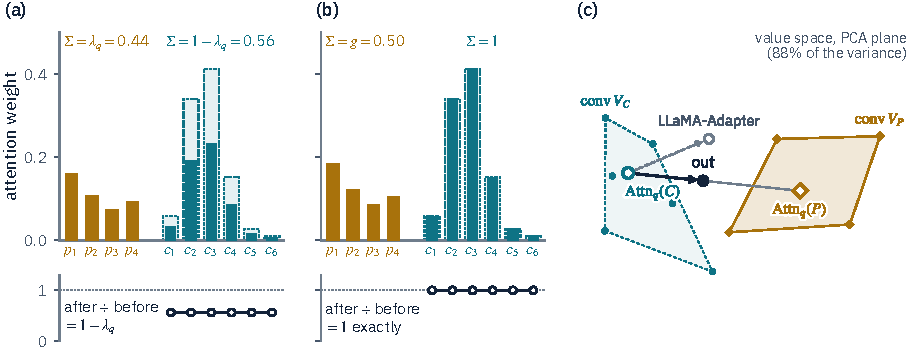
\includegraphics[width=\linewidth]{figures/prefix}
\caption{\textbf{A prefix is a gate} (\thmref{Theorem}{VI.5}). One query $q$ attends to six content tokens $C$ and four prefix tokens $P$, all seeded synthetic data. (a)~Prefix tuning \citep{li2021prefix}, one softmax over $P\uplus C$. The prefix (ochre) takes the mass $\lambda_q=Z_q(P)/(Z_q(P)+Z_q(C))$, and each content weight (teal) is its value without the prefix (dashed outline) times $1-\lambda_q$. The strip below plots the ratio after/before for every content token; it is the same for all six, so the content weights keep their ratios and their order (part~(c), due to \citet{petrov2023prompting}). (b)~LLaMA-Adapter \citep{zhang2023llama} normalises $P$ and $C$ separately and adds the prefix branch with a gate $g$: the prefix weights sum to $g$, and the content weights equal the no-prefix ones exactly (part~(d)). (c)~The value vectors projected on their two leading principal axes, with the hulls of the content values (dashed) and of the prefix values (ochre). The prefix-tuning output (black dot) lies on the segment from $\mathrm{Attn}_q(C)$ to $\mathrm{Attn}_q(P)\in\mathrm{conv}\,V_P$, the fraction $\lambda_q$ of the way (parts~(b) and~(c); the identity~(b) is due to \citet{he2021unified}), and a larger $\lambda_q$ moves it further towards the prefix hull. The LLaMA-Adapter output $\mathrm{Attn}_q(C)+g\,\mathrm{Attn}_q(P)$ (open grey) is an additive step that leaves the segment. The rigidity holds within one layer, relative to the same layer without the prefix: prefixes at lower layers change the queries, keys and values of higher ones. The values used are in \S\ref{app:repro-figures}.}
\label{fig:prefix}
\end{figure}

\begin{theorem}{VI.5}{attention is a homomorphism followed by a perspective map; known in part}
Fix a query $q$. Multisets of key--value pairs form a commutative monoid under $\uplus$. Define
\[\Sigma_q(K)=\Big(\sum e^{\langle q,k\rangle/\sqrt d},\ \sum e^{\langle q,k\rangle/\sqrt d}\,v\Big).\]

(a) $\Sigma_q$ is a monoid homomorphism into $(\R_{\ge0}\times\R^{d_v},+)$, landing in $\{Z>0\}\cup\{(0,0)\}$. On
nonempty multisets, $\mathrm{Attn}_q=\pi\circ\Sigma_q$ with the partial map $\pi(Z,S)=S/Z$, defined for $Z>0$.

(b) \textbf{Prefix is a gated parallel adapter.} For nonempty $P$ and $C$,
\[\mathrm{Attn}_q(P\uplus C)=(1-\lambda_q)\,\mathrm{Attn}_q(C)+\lambda_q\,\mathrm{Attn}_q(P),\qquad
\lambda_q=\frac{Z_q(P)}{Z_q(P)+Z_q(C)}.\]

(c) \textbf{Per-layer pattern rigidity.} Within a single layer, for fixed $q$ and a fixed content multiset $C$: the
content attention weights are multiplied by $1-\lambda_q$, their ratios are unchanged, and the output lies on the segment
from $\mathrm{Attn}_q(C)$ to $\mathrm{Attn}_q(P)\in\operatorname{conv}V_P$, where $V_P$ is the set of prefix values. This
rigidity is relative to the same layer's computation without the prefix; it is relative to the pretrained pattern only at
the lowest prefixed layer. Lower-layer prefixes change the queries and the content keys and values of higher layers, so
attention patterns at the level of the network are \emph{not} rigid (\citealp[§6]{petrov2023prompting}; the same authors
show that prefix-tuning a pretrained transformer can be a universal approximator, \citealp{petrov2024prompting}).

(d) \textbf{LLaMA-Adapter} normalises $P$ and $C$ separately and adds a zero-initialised gate. It computes
$\mathrm{Attn}_q(C)+\tanh(g_l)\,\mathrm{Attn}_q(P)$, with one gate per head in the paper; HF PEFT uses one raw
zero-initialised scalar per layer, without $\tanh$. It uses two perspective maps, leaves the content weights exactly
unchanged, and is pointed at $g=0$. Its prompt keys and values are the frozen $W_k,W_v$ applied to one learned prompt per
adapted layer, and it acts in the top layers only.

(e) \textbf{Prompt $\to$ deep prefix in causal decoders.} Assume that the soft prompt comes first, that attention is
causal, and that content positions are offset by the prompt length $m$ in both methods (as HF PEFT does via
\texttt{cache\_position}). Then at every layer the states at prompt positions depend only on $p$, and
$h:p\mapsto(K_j(p),V_j(p))_j$ satisfies
\[\Phi\circ\rho_{\mathrm{prefix}}\circ h=\Phi\circ\rho_{\mathrm{prompt}}\]
as functions of the content tokens, read at content positions. The two methods live on different extensions, so this is
an arrow of the unpointed slice over the realisation $C^\infty(X_{\mathrm{content}},Y_{\mathrm{content}})$, not of
$\Meth$. Under RoPE without the offset, a different $h$ works: rotate each prefix key by $-m$ (positions
$-m,\dots,-1$). For additive relative biases (ALiBi, T5) the answer depends on how the implementation places the prefix
keys. The construction does not apply in bidirectional encoders of depth $\ge2$.

(f) \textbf{Obstructions.} Call a head \emph{standard} if it is vanilla softmax attention without torch-style
\texttt{add\_bias\_kv} (which would absorb a one-token prefix), \texttt{add\_zero\_attn}, learned attention sinks or
softmax-plus-one. On length-one contexts, every weight setting of a standard head is affine in $x$. Some prefix makes the
prefixed head non-affine on length-one contexts iff $W_o\ne0$ and ($W_q\ne0$ or $W_k^\top b_q\ne0$); for bias-free heads,
iff $W_o\ne0$ and $W_q\ne0$. For such frozen weights and generic prefixes the prefixed head is not affine, because the
gate $\lambda(x)$ is not constant. So prefix tuning and P-tuning v2 are not box-locally mergeable into a standard head.
When $W_oW_v\ne0$, no prefix is neutral, so prompt and prefix tuning are unpointed.
\end{theorem}

The identity is standard. Part (b) is due to \citet{he2021unified}; see also \citet{chen2022inducer}. Part (c) and the
soft-prompt-to-prefix map in (e) are due to \citet[§2.2 and §6]{petrov2023prompting}, informally already
\citet[§7.2]{li2021prefix}. LLaMA-Adapter is \citet{zhang2023llama}, P-tuning v2 is \citet{liu2021p}, and prompt tuning
is \citet{lester2021power}; on what prompts can express, see \citet{wang2023universality}. Ours are the monoid
organisation, the explicit position hypotheses and the slice-category typing of (e).

\noindent\labelsf{Num}\enspace On a 3-layer, 2-head causal decoder, prompt-to-prefix agreement is $9\times10^{-16}$ with
RoPE and the offset, against $1.3$ without it and $2\times10^{-15}$ with keys rotated by $-m$. A head with $W_o=0$ stays
affine although $W_q^\top W_k\ne0$, and one with $W_q\ne0$, $W_q^\top W_k=0$ does not (referee replication). The identities
(a)--(d) and the non-affinity in (f) are checked to rounding error (Appendix~\ref{app:repro}); Figure~\ref{fig:prefix}
draws them for one query.

\begin{explains}
At the lowest prefixed layer the content attention equals the pretrained one, rescaled by $1-\lambda_q$. At higher layers
it changes only through the modified inputs, to first order additively in each position
\citep[§6]{petrov2023prompting}, so new query--key interactions cannot be imposed directly at a layer. No network-level
impossibility follows. LLaMA-Adapter's zero-init attention is a structural change; categorically, its contribution is
\emph{pointedness}. Prompt tuning maps into P-tuning v2 in causal decoders. \citet{petrov2023prompting} and
\citet{li2021prefix} assert that the inclusion is strict. It is strict in a one-layer, one-token example, where a prompt
fixes the prefix value as a function of its key, and we do not prove the generic statement. Encoders remain open.
\end{explains}


% ------------------------------------------------------------------------------------------------
\subsubsection{Where each method lands}\label{sec:merge-summary}

Table~\ref{tab:merge-summary} collects the verdicts of this exposé.

\begin{table}[tp]
\centering\footnotesize\renewcommand{\arraystretch}{1.15}
\caption{Extensions and their merge types. The verdicts are box-local (\thmref{Definition}{VI.1}), and the attention
results are per layer.}\label{tab:merge-summary}
\begin{tabularx}{\linewidth}{@{}>{\raggedright\arraybackslash}p{0.18\linewidth}>{\raggedright\arraybackslash}p{0.21\linewidth}>{\raggedright\arraybackslash}p{0.16\linewidth}>{\raggedright\arraybackslash}p{0.07\linewidth}>{\raggedright\arraybackslash}X@{}}
\toprule\headrow
\textbf{Method} & \textbf{What it adds} & \textbf{Neutral point} & \textbf{Merge} & \textbf{Reason}\\
\midrule
LoRA, DoRA, OFT, HRA & nothing; weight-space reparametrisations & their pointing in $\Meth$ & $\mathsf{M1}$ &
nonlinearity on the parameter side; $\mu=\rho$\\
(IA)$^3$ on $k$, $v$ & output scaling of $W_K$, $W_V$ & $\ell=\mathbf 1$ & $\mathsf{M1}$ & R1\\
(IA)$^3$ on the FFN & input scaling of $W_{\mathrm{down}}$ & $\ell=\mathbf 1$ & $\mathsf{M1}$, $\mathsf{M1}{\rightarrow}$
& R1 into $W_{\mathrm{down}}$; R4 into $W_{\mathrm{up}}$ under SwiGLU, R3 under ReLU with $\ell\ge0$\\
SSF & scale and shift after a box & $\gamma=\mathbf 1$, $\beta=0$ & $\mathsf{M1}{\rightarrow}$ & R1 into the preceding box
if it has a bias slot\\
LN-tuning & new values of existing $\gamma,\beta$ & the pretrained values & $\mathsf{M1}$ & in place; folding forward
needs pre-LN, and $\beta$ a bias slot\\
linear adapter parallel to one box & $sUDx$ beside $W_0x$ & $U=0$ & $\mathsf{M1}$ & \thmref{Proposition}{VI.4}(a): it is
LoRA\\
serial linear adapter & $(I+UD)$ after $W_0$ & $U_0D_0W_0=0$ & $\mathsf{M1}$ & \thmref{Proposition}{VI.4}(b)\\
Houlsby, Pfeiffer, nonlinear parallel adapters & $U\sigma(D\,\cdot)$ & $U=0$; Houlsby's init starts near it &
$\mathsf{M}\infty$ & non-affine edit, \thmref{Theorem}{VI.3}(c)\\
routed mixtures (MoLE, LoRAMoE, X-LoRA) & input-dependent gates over LoRA modules & varies & $\mathsf{M}\infty$ &
\thmref{Theorem}{VI.3}(c); mergeable if the gate is constant\\
AdapterFusion, LST & a gated mix of nonlinear adapters; a side network & none & $\mathsf{M}\infty$ & non-affine edit,
\thmref{Theorem}{VI.3}(c)\\
LoReFT & identity box with a rank-$\le r$ affine edit, at selected positions & $W=R$, $b=0$; pyreft's init misses it &
$\mathsf{M}\infty$ & position-selective, outside \thmref{Theorem}{VI.3}(a); no merge known\\
prefix tuning, P-tuning v2 & key--value pairs in every layer & none, generically & $\mathsf{M}\infty$ & box-locally,
\thmref{Theorem}{VI.5}(f)\\
prompt tuning & soft tokens at the input & none, generically & $\mathsf{M}\infty$ & a deep prefix in causal decoders
(\thmref{Theorem}{VI.5}(e)), so \thmref{Theorem}{VI.5}(f)\\
LLaMA-Adapter & a separately normalised, gated prompt in the top layers & $g=0$, \thmref{Theorem}{VI.5}(d) &
$\mathsf{M}\infty$ & as in \thmref{Theorem}{VI.5}(f), once the prompt has two or more tokens\\
QLoRA, LoftQ & nothing; LoRA on a quantised base & pointed off $\theta_0$, with a defect & $\mathsf{Mq}$ &
\thmref{Theorem}{VI.3}(d), \thmref{Proposition}{V.2}(d); QA-LoRA stays on the grid\\
\bottomrule
\end{tabularx}
\end{table}

The verdicts are box-local, and the attention results are per layer. Two questions remain open
(Exposé~\ref{sec:analogy}): whether prefix tuning is non-mergeable for the whole network, and whether prompt tuning is
strictly weaker than P-tuning v2 in general causal decoders, together with how the two relate in encoders.
